\chapter{Конструкторский раздел}
\label{cha:design}
В данном разделе будет рассмотрена схема алгоритма Винограда и описаны его параллельные реализации.

\section{Схемы алгоритмов}
\label{sec:schemes}
На рисунке \ref{fig:winograd} представлена схема алгоритма Винограда умножения матриц.
\begin{figure}
	\centering
	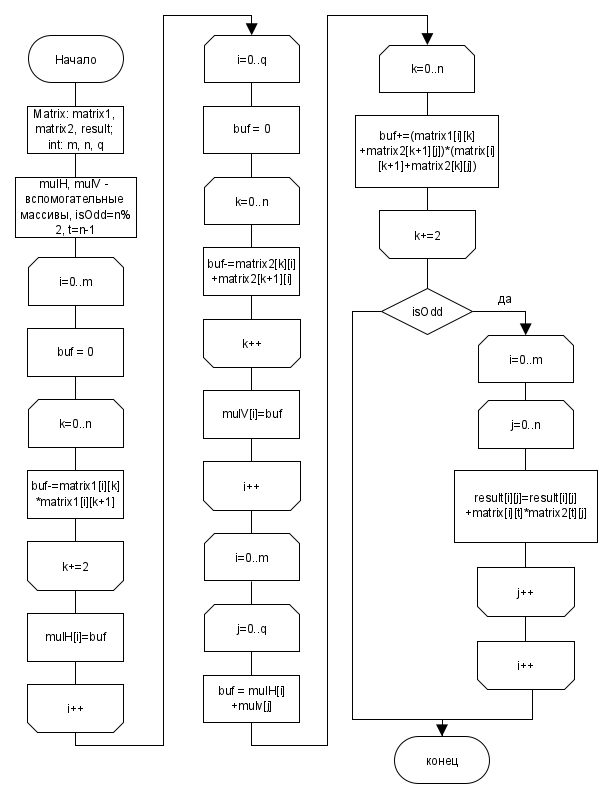
\includegraphics[width=0.8\linewidth]{src/winograd}
	\caption[Алгоритм Винограда]{Алгоритм Винограда}
	\label{fig:winograd}
\end{figure}

\section{Распараллеливание программы}
В первой параллельной реализации параллельно выполняется подсчёт строк результирующей матрицы, в главном потоке подсчитываются вспомогательные массивы mulV и mulH, после чего он создаёт потоки, формирующие результирующую матрицу, передаёт им параметры, и после их завершения, в случае если размеры матрицы нечётные, дополняет ее.
\par Во второй реализации параллельно рассчитываются массивы mulH и mulV, так как их подсчёт не зависит от их собственных значений, то их можно распараллелить. Главный поток создаёт рабочие потоки, передаёт им параметры и определяет границы участков массивов, над которыми они будут работать, эти потоки подсчитывают значения массивов, после чего управление возвращается к главному потоку.

\section{Вывод}
\label{sec:design_conclusion}
В данном разделе была рассмотрена схема алгоритма Винограда умножения матриц, описаны 2 метода его параллельной реализации.